\chapter{Design}
\label{cha:design}

\section{Architecture}
\label{sec:design-architecture}
Omni will use a microservices architecture. This enables a highly distributed and scalable system that can respond dynamically to changes in incoming requests.
The approach should make use of common industry standards and technology as well as be portable across cloud providers. The aim is to build Omni cloud-natively so that it could scale exponentially in the case of a "viral" moment.
mni will be primarily designed using the microservices architecture. This enables a highly distributed and scalable system, which is able to respond to changes in incoming requests dynamically. 
The approach should make use of common industry standards and technology as well as be portable across cloud providers. The aim is to build Omni cloud-natively so that it could scale exponentially in the case of a "viral" moment.

\subsection{Kubernetes and Containerisation}
\label{sec:design-system-kubernetes}
Kubernetes is an orchestration tool which enables the management of pods across clusters. A cluster is one or more nodes (physical machines) connected together, possibly across different data centres or even regions, which run workloads.


\begin{figure}[htbp]
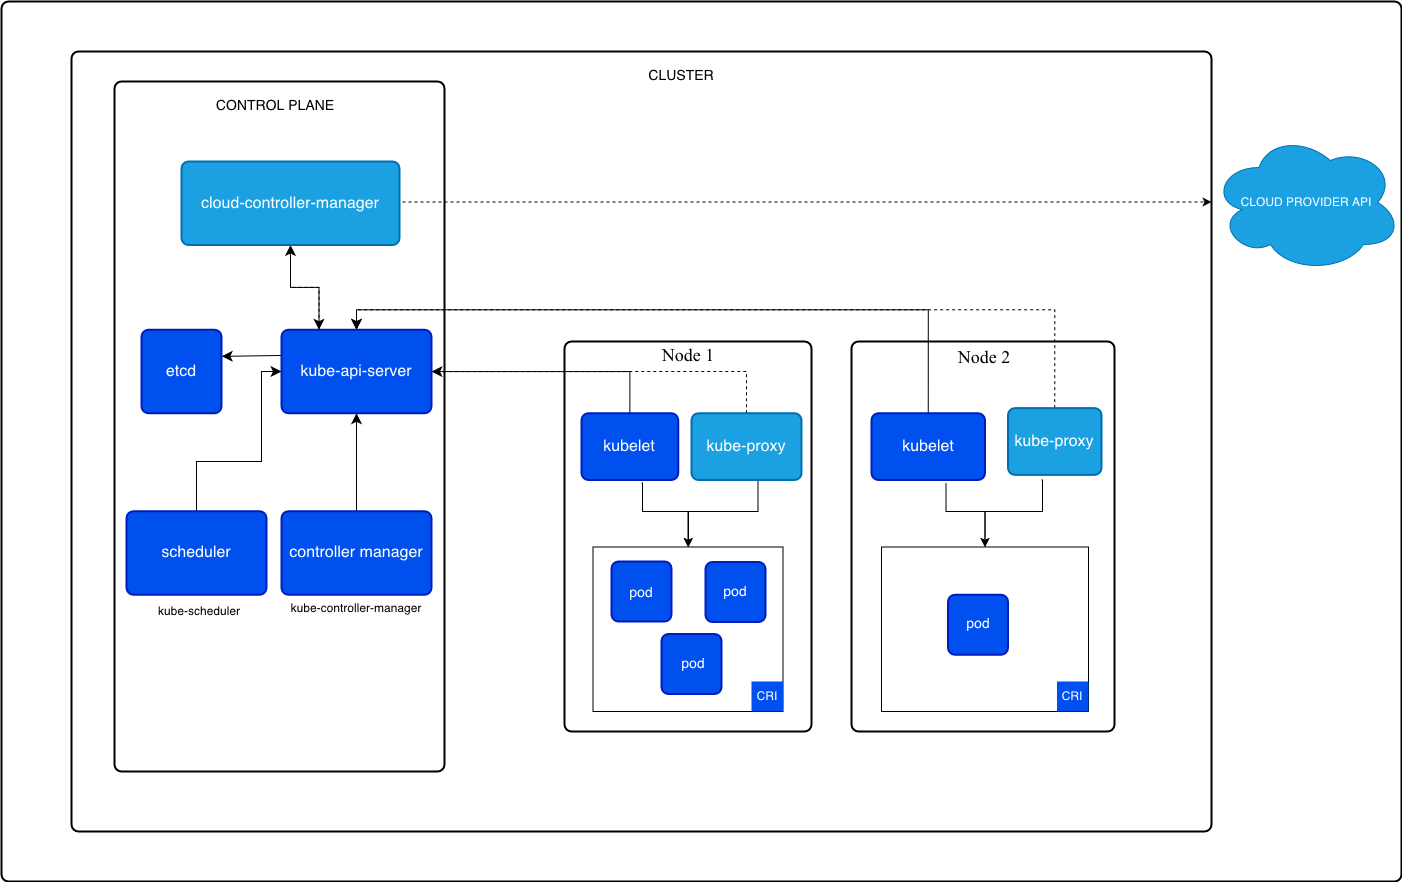
\includegraphics[width=12cm]{k8s-arch.png}
\centering
\caption{Kubernetes Architecture}
\end{figure}

Kubernetes manages the lifecycle of pods using the industry standard health check endpoints:
\begin{itemize}
    \item \texttt{/healthz} - General health of the pod
    \item \texttt{/readyz} - Whether the pod is ready to receive requests
    \item \texttt{/livez} - Whether the pod is alive and should be running
\end{itemize}

Using these endpoints, Kubernetes deployments can monitor the pods (a pod is a running unit usually containing one but sometimes more containers) they have spawned and, if any of them die, for example, if they crash, auto-heal and spawn a replacement.
Deployments can also be configured to scale up the number of pods they run when certain limits are reached. The possibilities are endless, but some common examples could be CPU usage on a particular node or the number of requests received per time period.

This is what makes Kubernetes super powerful. Combining auto-healing and management of ephemeral pods with autoscaling leads to solutions that are highly adaptable to any scenario.
For this reason, Omni will be designed to run natively in Kubernetes. This means that I will need to create containerised applications to run the platform.

Containerisation is the process of modifying an application to run within a container. A container is a self-contained module that can be run without needing to worry about its dependencies or setup. For example, if an application has a dependency on a particular version of Linux with a certain library installed, containerisation will mean that the user running the container can execute the application on any supported OS without needing to worry about the dependencies.

The other added benefit of containers is that the execution environment only needs to contain the compiled binary. Rather than the host machine needing to compile the binary or a CI/CD pipeline creating many binaries for various operating systems, we can use one container, which contains only the compiled binary for the container's OS.

So, for Omni, the application(s) should be containerised and ready for deployment to a Kubernetes cluster in any of the major cloud providers (as well as bare-metal solutions).
Kubernetes is a perfect fit for the microservices architecture described in Section 1: It simplifies the management of individual containers and their lifecycles and provides auto-scaling, rollbacks, service discovery, security and portability. Because of this, Kubernetes is ideal for maintaining scalable and reliable microservice-backed platforms.

\section{Database}
\label{sec:design-system-database}
Omni's database needs to scale horizontally across many machines to handle potentially hundreds of thousands or even millions of users. Database sharding will be needed to ``build scalable, fault-tolerant, and efficient database architectures'' \citep{shethiya2025load}.
In order to accomplish successful database sharding, one of the problems that needs to be solved is how to locate data. Formally:
\begin{quotation} % TODO: Make this not indent weirdly
Given N nodes (where N is sufficiently large), how can a backend locate a specific piece of data whilst preventing a worst case $O(N)$.
\end{quotation}
Ideally, we want data retrieval to be of the order $O(1)$, where a backend knows exactly where to look to find a piece of data that we want to retrieve.

\subsection{Snowflake IDs} 
\label{sec:design-system-database-snowflake}
Luckily, this problem has been solved for us. Engineers at Twitter (now X) faced this same problem and came up with an intuitive solution: snowflake IDs. Snowflake IDs are a type of ID that not only uniquely describes a piece of data but also its locality: where it is stored \citep{2010snowflake}. This enables data to be sharded across many database instances whilst retaining a look-up time with a complexity of $O(1)$.
Snowflake IDs are unique 64-bit integers with the following properties:
\begin{itemize}
    \item The first bit is locked to 0, which ensures that all snowflake IDs are positive. Treating them as signed or unsigned does not matter.
    \item The following 41 bits are dedicated to be a timestamp. This is the time that the ID was created and is based on a custom epoch (rather than the UNIX epoch) to increase the range.
    \item Following the timestamp, each ID has a 10-bit Node ID. This represents the location where a piece of data has been stored.
    \item Finally, we have a 12-bit Sequence ID. This prevents collisions between IDs created for the same Node ID and Timestamp.
\end{itemize}
\ref{tab:snowflake} shows the final structure of the 64-bit Snowflake ID.

\begin{table}[htbp]
\centering
\begin{tabular}{|l|l|l|l|}
\hline
1 bit unused & 41 bit timestamp & 10 bit node id & 12 bit sequence id \\ \hline
\end{tabular}
\caption{Snowflake ID Structure}
\label{tab:snowflake}
\end{table}

Using these Snowflake IDs, it becomes obvious how to store data across many nodes while retaining an efficient retrieval mechanism. A backend only needs to inspect the bits representing the snowflake's node to determine where to route its request. Using 10 bits for this value also allows us to scale up to 1024 nodes, which should be plenty for even the largest social media networks.

When using Snowflake IDs, the key concern is ensuring that only a single object in a given backend can create the IDs and that each backend is assigned a unique Node ID (even if multiple Node IDs are stored in the same database shard). 
This prevents ID collisions during generation, rather than using a 128-bit ID like the one specified in the RFC 4122 UUID specification \citep{rfc4122}.

\subsection{Database Implementation}
\label{sec:design-system-database-implementation}
A classic SQL database will suit our needs since the data we will store in a social media network is structured, where the relationships between users, posts, and comments are known.
The added flexibility of a NoSQL database, whilst attractive for sharding, is not warranted for such a platform, and a more strict and structured scheme should bring benefits in the long run compared to developer experience and stability.

Given this directive, some natural choices are SQLite and MySQL/MariaDB. They are both simple and robust; however, MySQL/MariaDB is better suited for this particular application with a single (sharded) database. In lightweight/mobile applications, SQLite is the preferred option.

As mentioned above in Section \ref{sec:design-system-database-snowflake}, the database will be sharded so that the load of multiple backends accessing data from the database is balanced across multiple servers. 
This allows databases to be located in separate regions and balances the load across multiple servers.
Another option to balance the load on the database is to use read replicas, where there is one primary node and many read replicas, which are a copy of the primary node.
This setup is perfect for read-heavy applications, as read requests are distributed across the replicas.
It also brings the benefit of higher availability, as all servers have the same database, so if the primary node fails, other nodes can be promoted to receive write requests.
Replication does bring a write bottleneck where only one server can process writes to maintain ACID compliance. 

Overall, sharding is the better option for the Omni platform due to the write bottleneck and the potentially massive amount of data that will be stored in the database.
A future improvement would be to use a hybrid approach, where some things, like the user profile data, which is not expected to receive many writes, are stored in a replicated database, whereas post and comment data is stored in a sharded database to prevent a bottleneck when writing.


\section{Backend}
\label{sec:design-system-backend}
Omni has a couple of requirements for the backend:
\begin{itemize}
    \item The backend needs to be able to service both users interacting with the frontend as well as via an API
    \item The backend must be able to scale to meet the needs of the incoming requests
\end{itemize}
Considering these requirements, the backend must be designed to scale efficiently. A social media platform expects to receive a lot more read requests than write requests.
Splitting the backend into multiple microservices that can scale to demands independently puts the platform in the best position to maintain availability and reliability. 
One way to achieve this is to use separate microservices for read and write requests. This allows us to scale the read service to use many more instances than the write service during periods of high usage. 

By adopting this approach, we can also split other sections of the application into separate microservices.
For example, we could use an authentication service that is only responsible for logging users in and providing them with a JWT token for future requests.
There is no limit to the granularity of the microservices used.
However, there will likely be a limit of diminishing returns where further breaking down microservices does not lead to significant performance improvements compared to the effort spent creating them.

\subsection{Omni Microservices}
\label{sec:design-system-backend-microservices}
Based on the discussion in Section \ref{sec:design-system-backend} above, Omni's backend is split into three different microservices, built using GoLang:
\begin{itemize}
    \item OmniRead, which will handle purely read API requests with no side effects
    \item OmniWrite, which will handle any API request that modifies the \\database
    \item OmniAuth, which will handle authenticating a user when they log in as well as provisioning JWT tokens
\end{itemize}

We do not want separate API endpoints for each service. To route requests to the correct microservice, we will use a layer 4 load balancer. Because requests are balanced based on their HTTP method and path (GET requests are for OmniRead, /login requests are for OmniAuth, and everything else is for OmniWrite), a layer 4 load balancer, which operates at the application layer, is preferred over a lower-level layer 7 load balancer, which operates on TCP/UDP packets.

\section{Frontend}
\label{sec:design-system-frontend}
Similar to how multiple microservices serve the backend, the website will be served by a separate microservice that is only responsible for rendering page content.
Any data the frontend service (OmniView) requires will be retrieved by calling the backend inside the Kubernetes cluster. Kubernetes allows pods inside the same cluster to communicate with each other via standard HTTP requests.
As the website is not the main focus of this project, and a social media platform inherently does not have much onscreen interaction (instead, they are traditionally comprised of many pages linked together), the website will be built with a combination of HTMX (served via the GoLang microservice), TailWindCSS for styling, and AlpineJS for the limited amounts of more complex interaction that is required.


\subsection{UI Design}
\label{sec:design-ui}
% TODO: Add images and initial design here

\section{Tech Stack}
\label{sec:design-review}
The Omni microservices will be built using GoLang. This is a fast language with excellent concurrency features, making it ideal for web servers and APIs.
The SQLc library will automatically generate the database layer from the SQL migrations and queries to connect to the database from within Go.
Letting a code generation framework create this code automatically ensures that the database and the microservices will always be in sync, and any errors caused by new migrations will be flagged as type errors during building. 

As mentioned in Section \ref{sec:design-system-frontend}, the website will use HTMX, TailwindCSS, and AlpineJS. HTMX is a lightweight JavaScript framework that can be used for client-side interactivity as an alternative to ReactJS or NextJS.
Using HTMX, you can dynamically update portions of the page by serving partial HTML snippets from the webserver. This can be used, for example, to add a new post to a list of posts dynamically.

MariaDB is the database of choice for the reasons mentioned in Section \ref{sec:design-system-database-implementation}, and Kubernetes will be used to orchestrate the workloads being run. I have built a custom Kubernetes cluster running across 3 Raspberry Pis which will be used for testing, but there is nothing stopping the same deployments to be used in a cloud-based Kubernetes environment like GKE, AKS or EKS (from Google Cloud, Microsoft Azure and Amazon Web Services respectively).
